\documentclass{../cssheet}

%--------------------------------------------------------------------------------------------------------------
% Basic meta data
%--------------------------------------------------------------------------------------------------------------

\title{Schubspiegelung}
\author{Prof. Dr. Christian Spannagel}
\date{\today}
\hypersetup{%
    pdfauthor={\theauthor},%
    pdftitle={\thetitle},%
    pdfsubject={Aufgabenblatt Geometrie},%
    pdfkeywords={geometrie}
}


%--------------------------------------------------------------------------------------------------------------
% document
%--------------------------------------------------------------------------------------------------------------

\begin{document}
\printtitle

In diesem Aufgabenblatt untersucht ihr, was passiert, wenn man drei Achsenspiegelungen verkettet, wenn die drei Geraden nicht im Büschel liegen.

\textbf{Aufgabe 1 (Sonderfall):}  Wir betrachten zunächst einen Sonderfall: Zwei Achsen $a$ und $b$ sind parallel zueinander, die dritte Achse $c$ dazu senkrecht. Die Abbildung ist $a\circ b\circ c$.
\begin{center}
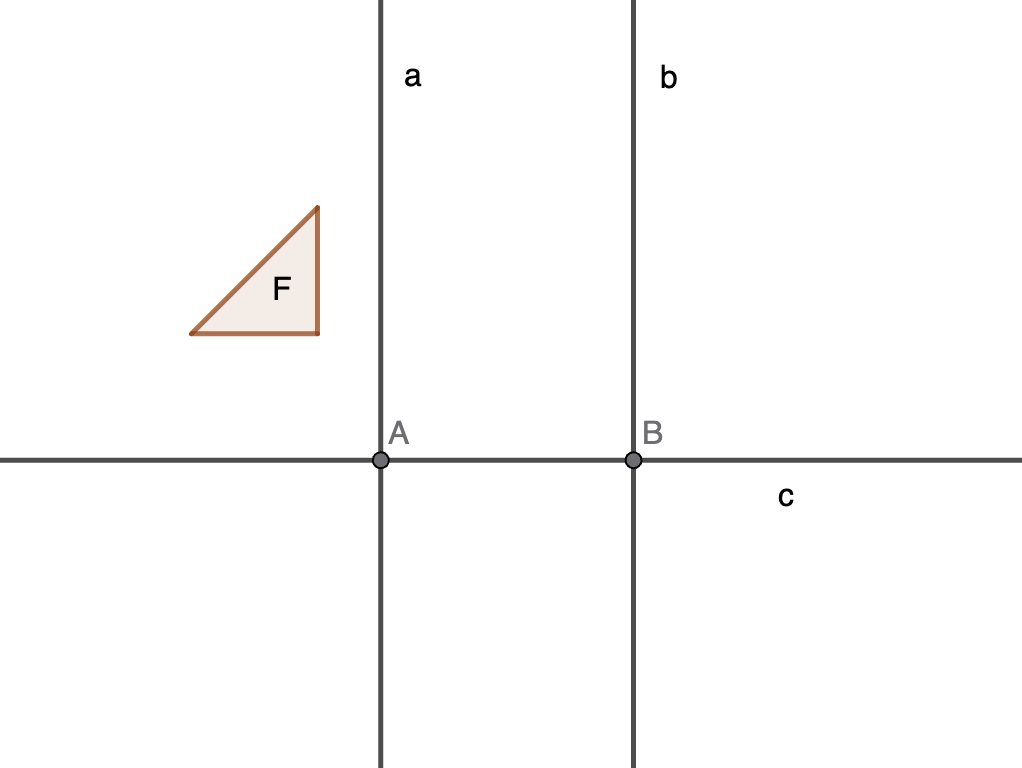
\includegraphics[width=8cm]{schubspiegelung.png}
\end{center}

\begin{enumerate}[a)]
\item Bildet die Figur $F$ ab.
\item Durch welche äquivalenten Abbildungen könnt ihr die Abbildung $a\circ b\circ c$ ersetzen?
\end{enumerate}

\textbf{Aufgabe 2 (Verallgemeinerung):} 
\begin{enumerate}[a)]
\item Im allgemeinen Fall bilden drei Geraden ein Dreieck. Beweist, dass eine Spiegelung an drei solchen Geraden eine Schubspiegelung ist.
\item Macht das gleiche nochmal für den Fall, dass zwei der drei Geraden parallel sind.
\end{enumerate}

\textbf{Aufgabe 3 (Eigenschaften):}  Welche Eigenschaften hat die Schubspiegelung? Ist sie längentreu, winkeltreu, parallelentreu, geradentreu? Hat sie Fixpunkte, Fixgeraden oder Fixpunktgeraden?

\vspace*{10mm}
Die Aufgaben orientieren sich an: Krauter, S. \& Bescherer, C. (2013). \emph{Erlebnis Elementargeometrie} (2. Aufl.). Berlin, Heidelberg: Springer. S.~31--33


\printlicense

\printsocials

\end{document}
